\documentclass{article}
\usepackage{graphicx}
\usepackage{float}
\usepackage{titlesec}
\usepackage{datetime}
\usepackage{geometry}
\usepackage{placeins}
\usepackage{minted}
\usepackage{xcolor}
\usepackage{listings}
\usepackage{caption}
\usepackage[document]{ragged2e}
\usepackage[hidelinks]{hyperref}
\usepackage{enumitem}
\usepackage{booktabs}
\geometry{
 a4paper,
 left=25mm,
 top=25mm,
 }
\captionsetup{hypcap=false} 
\newdateformat{daymonthyear}{\THEDAY .\THEMONTH .\THEYEAR}
\title{
  \centering
  
\includegraphics[width=\textwidth]{src/images/logo_PWr_kolor_poziom.png}\\
  \fontsize{28pt}{30pt}\selectfont Programowanie efektywnych algorytmów\\
  \fontsize{14pt}{30pt}\selectfont Problem komiwojażera (TSP)}
\author{Krzysztof Zalewa}
\date{\daymonthyear\today}
\renewcommand*\contentsname{Spis treści}
\renewcommand{\figurename}{Rysunek}
\renewcommand{\listingscaption}{Fragment kodu}
\begin{document}
    \maketitle
    \pagebreak
    \tableofcontents
    \FloatBarrier
    \raggedright
    \section{Specyfikacja sprzętu użytego do badań}
      Badania zostały wykonanie na komputerze stacjonarnym o specyfikacji: \linebreak
      \textbf{Procesor:} Intel(R) Core(TM) i7-9700K CPU \linebreak
      \textbf{Zegar:} 3.60GHz \linebreak
      \textbf{Wielkość pamięci RAM:} 32,0 GB (dostępne: 31,8 GB) \linebreak
      \begin{figure}[ht]
        \centering
        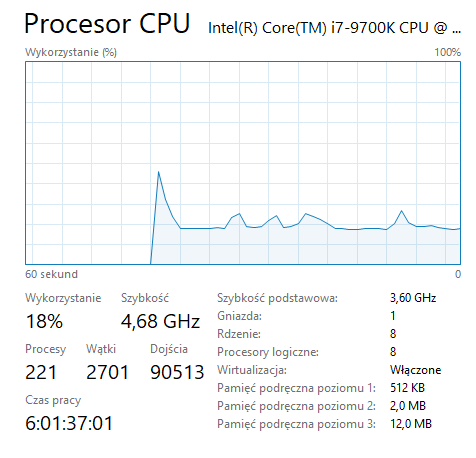
\includegraphics[width=\textwidth]{src/images/Zurzycie_procesora_Tabu.png}
        \caption{Zurzycie procesora w trakcie wykonywania algorytmu Tabu search}
        \label{fig:procTabu}
      \end{figure}
      \FloatBarrier
    \section{Instancje użyte w badaniach}
      Do badań użyłem macierzy z \hyperref[src:TspLib]{TspLib[~\ref*{src:TspLib}]} \linebreak
      \textbf{Macierze symetryczne} - rat99.tsp,pr152.tsp,ts225.tsp oraz pr264.tsp \linebreak
      \textbf{Macierze asymetryczne} - ftv33.atsp,ftv64.atsp,\hyperref[txt:explanation1]{kro124p.atsp*}  oraz ftv170.atsp \linebreak
      Gdzie najleprze znane rozwiązania to :
      \begin{table} 
        \centering
        \begin{tabular}{|r|r|r|r|r|r|r|r|r|}
          \hline
          &\multicolumn{4}{|c|}{Symetryczne} & \multicolumn{4}{|c|}{Asymetryczne} \\ \hline\
          Instancje & rat99 & pr152 & ts225 & pr264 & ftv33 & ftv64 & \hyperref[txt:explanation1]{kro124p*}  & ftv170 \\ \hline
          & 1211 & 73682 & 126643 & 49135 & 1286 & 1839 & 36230 & 2755 \\ \hline
        \end{tabular}
        \caption{Optymalne wyniki z TspLib}
        \label{txt:opt}
      \end{table}
      \FloatBarrier
      \label{txt:explanation1}
      * Mimo tego że powinna być to instancja o 124 wierzchołkach po konwersji 
      otrzymuję tylko 100 wierzchołków. Pozostałe instancje konwertują się poprawnie.     
    \section{Tabu search}
      \subsection{Opis Algorytmu}
        Algorytm tabu search jest algorytmem metahurystycznym służącym do rozwiązywania
        problemów optymalizacyjnych. Algorytm ten przechowuje część otrzymanych wcześniej 
        rozwiązań w tablicy tabu. Takie podejście sprawia że szansa na ponowne wybranie
        tego samego rozwiązania znacznie maleje. Sprawia to też że jest mniejsza szansa 
        na utknięcie w pętli. Algorytm ten można jeszcze usprawnić poprzez dodanie 
        warunku krytycznego i strategii dywersyfikacji.\linebreak
        \textbf{Warunek krytyczny: } Jeżeli otrzymana wartość jest mniejsza
        od najlepszej do tej pory znalezionej wartości ale ścieżka znajduje się
        w tabu to i tak przypisujemy obecną wartość do najlepszej.\linebreak
        \textbf{Strategia dywersyfikacji: } Jeżeli przez określoną liczbę iteracji algorytmu
        wartość się nie poprawiła zmieniamy wybraną ścieżkę. W mojej implementacji zmiana
        ścieżki polega na wylosowaniu nowej przy użyciu funkcji std::shuffle.
      \subsection{Badanie wpływu metody przeszukiwania sąsiedztwa} 
        W moim algorytmie zaimplementowałem dwie różne metody przeszukiwania sąsiedztwa.
        \begin{enumerate}
          \item Swap - Wybieram dwa wierzchołki i zamienia je ze sobą. W mojej implementacji
          sprawdzam wszystkie unikalne możliwości więc generuję n*(n-1)/n sąsiadów.
          \item Insert - wybieram wierzchołek i miejsce w tablicy. Wierzchołek kopiuje a następnie 
          usuwam z tablicy. Na koniec kopię wierzchołka wstawiam w wybrane miejsce. W mojej 
          implementacji obie wartości losuję. Wykonuję n*(n-1)/n losowań.
        \end{enumerate}
        \textbf{Hipoteza: } W tabu search metoda przeszukiwania insert powinna być znacznie lepsza
        niż swap.
        \textbf{Badania: } Wykonuję badania dla każdej z 8 instancji. Żeby otrzymać dobrą próbkę 
        badanie powtarzam cztero krotnie dla każdej instancji. Więc wykonuje (4*ASYM + 4*ASM)*4 * 2 = 64
        badań.
        \begin{table}
\begin{tabular}{|r|r|r|r|r|r|r|r|r|}
\hline
 & \multicolumn{4}{|c|}{Symetryczne} & \multicolumn{4}{|c|}{Asymetryczne} \\ \hline\
Rozmiar[Liczba wierzchołków] & 99 & 152 & 225 & 264 & 33 & 64 & 100 & 170 \\ \hline
Błąd wzgledny[\%] & 15.32 & 16.95 & 17.42 & 13.84 & 18.27 & 18.76 & 18.65 & 18.76 \\ \hline
\end{tabular}
\caption{Błędy w wynikach algorytmu dla macierzy symetrycznych i niesymetrycznych}
\label{tab:error_TsInsert}
\end{table}

        \begin{figure}[ht]
          \centering
          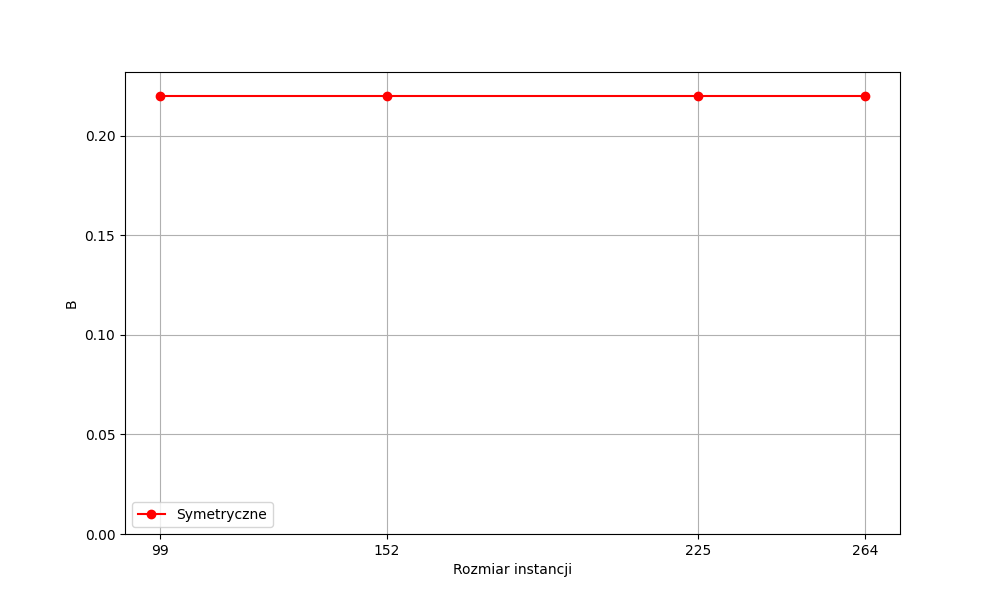
\includegraphics[width=\textwidth]{src/plots/symtest.png}
          \caption{Wyniki badań dla macierzy symetrycznych}
          \label{fig:symNeighg}
        \end{figure}
        \FloatBarrier
        \begin{figure}[ht]
          \centering
          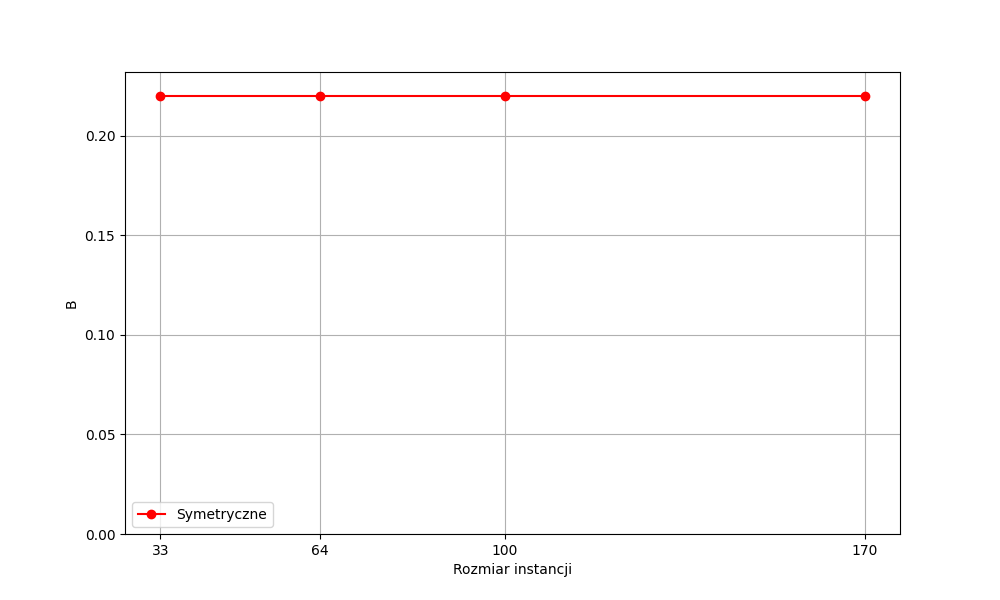
\includegraphics[width=\textwidth]{src/plots/asymtest.png}
          \caption{Wyniki badań dla macierzy asymetrycznych}
          \label{fig:asymNeighg}
        \end{figure}
        \FloatBarrier
        \textbf{Wnioski: }

      \subsection{Badanie wpływu metody tworzenia pierwszego rozwiązania}
        W moim algorytmie zaimplementowałem dwie różne metody tworzenia pierwszego rozwiązania.
        \begin{enumerate}
          \item Losowa - Pierwsze rozwiązanie jest zupełnie losowe. Najpierw tworzę wektor z liczbami
          od 0 do n - 1. Następnie na tym wektorze używam funkcji shuffle. 
          \item Nearest neighbour - Korzystam z wcześniej zaimplementowanego algorytmu NN. 
        \end{enumerate}
        \textbf{Hipoteza: } Wyniki dla metody losowej będą znacznie gorsze (Większy błąd wzgledny) od NN.
        Ale jest też niewielka szansa na wyniki będące bliżej optymalnego rozwiązania. Jednakże wykonanie
        wielu pomiarów powinno wykluczyć znaczne odstępstwa.\linebreak
        \textbf{Badania: } Podobnie jak w poprzednim przypadku wykonuje badania dla każdej z 8 instancji
        po 4 powtórzenia. Więc znowu wykonuje (4*ASYM + 4*ASM)*4 * 2 = 64\linebreak
        \begin{figure}[ht]
          \centering
          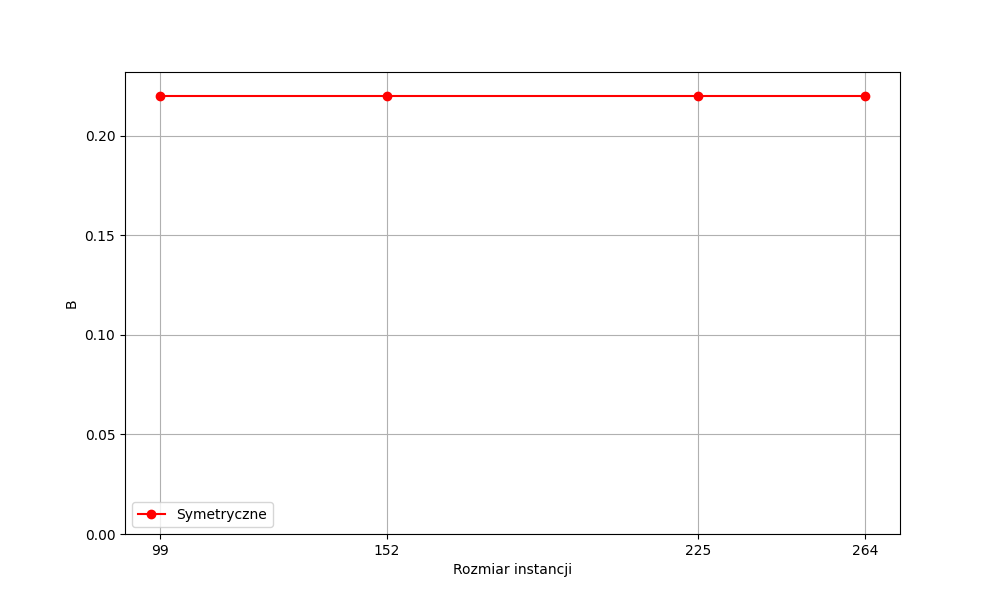
\includegraphics[width=\textwidth]{src/plots/symtest.png}
          \caption{Wyniki badań dla macierzy symetrycznych}
          \label{fig:symFirst}
        \end{figure}
        \FloatBarrier
        \begin{figure}[ht]
          \centering
          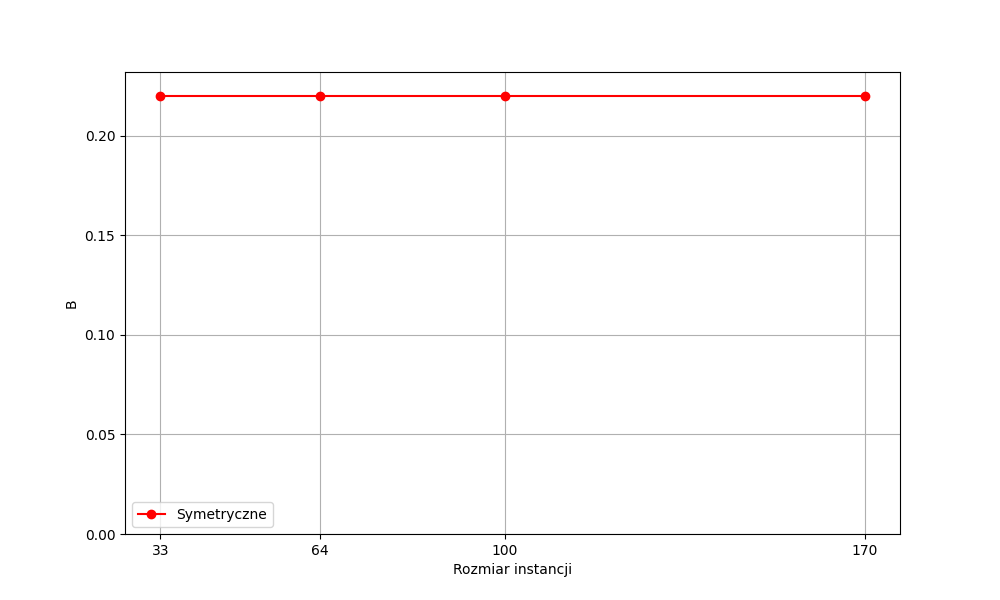
\includegraphics[width=\textwidth]{src/plots/asymtest.png}
          \caption{Wyniki badań dla macierzy asymetrycznych}
          \label{fig:asymFirst}
        \end{figure}
        \FloatBarrier
        \textbf{Wnioski: } 

      \subsection{Badanie wpływu ilości iteracji bez zmian}
        W mojej implementacji przekroczenie pewnej ilości bez zminay wyniku
        służy do dywersyfikacji. Do testów wybrałem wartości 25,50,75,100,125.\linebreak
        \textbf{Hipoteza: } Wraz ze wzrostem ilości iteracji bez zmian jakość
        rozwiązania też będzie rosła.\linebreak
        \textbf{Badania: } Dla każdej instancji testuje wszystkie 5 wartości. 
        Żeby otrzymać dobrą próbkę badanie powtarzam cztero krotnie dla każdej 
        instancji. Dla tego wykonuję (4*ASYM + 4*ASM)*5 * 4 = 160 badań.\linebreak

        \textbf{Wnioski: } 

      \subsection{Badanie wpływu długości tablicy tabu} 
        W mojej implementacji elementy pozostają w tablicy tak długo aż 
        ilość elementów w tej tablicy nie przekroczy pewnej liczby. Długość
        tablicy zależna jest od ilości wierzchołków (n * mnożnik).Do testów
        wybrałem wartości 0.5,0.4,0.3,0.2,0.1.\linebreak
        \textbf{Hipoteza: } Jakość rozwiązania powinna rosnąć kiedy długość
        tabeli tabu maleje. Jednakże zbyt mała wartość spowodować cykliczne 
        powracanie do już wygenerowanych rozwiązań.\linebreak
        \textbf{Badania: } Podobnie jak w ostatnim badaniu dla każdej instancji 
        testuje wszystkie 5 wartości. Żeby otrzymać dobrą próbkę badanie 
        powtarzam cztero krotnie dla każdej instancji. Dla tego wykonuję 
        (4*ASYM + 4*ASM)*5 * 4 = 160 badań.\linebreak

        \textbf{Wnioski: } 

      \subsection{Podsumowanie}
    \subsection{Simulated anealing}
      \subsection{Swap lub Insert}
        W moim algorytmie zaimplementowałem dwie różne metody przeszukiwania sąsiedztwa.
        \begin{enumerate}
          \item Swap - Wybieram dwa wierzchołki i zamienia je ze sobą. W mojej implementacji
          sprawdzam wszystkie unikalne możliwości więc generuję n*(n-1)/n sąsiadów.
          \item Insert - wybieram wierzchołek i miejsce w tablicy. Wierzchołek kopiuje a następnie 
          usuwam z tablicy. Na koniec kopię wierzchołka wstawiam w wybrane miejsce. W mojej 
          implementacji obie wartości losuję. Wykonuję n*(n-1)/n losowań.
        \end{enumerate}
        \textbf{Hipoteza: } W tabu search metoda przeszukiwania insert powinna być znacznie lepsza
        niż swap.
        \textbf{Badania: } Wykonuję badania dla każdej z 8 instancji. Żeby otrzymać dobrą próbkę 
        badanie powtarzam cztero krotnie dla każdej instancji. Więc wykonuje (4*ASYM + 4*ASM)*4 * 2 = 64
        badań. 

        \textbf{Wnioski: } 
      \subsection{NN lub random}
        W moim algorytmie zaimplementowałem dwie różne metody tworzenia pierwszego rozwiązania.
        \begin{enumerate}
          \item Losowa - Pierwsze rozwiązanie jest zupełnie losowe. Najpierw tworzę wektor z liczbami
          od 0 do n - 1. Następnie na tym wektorze używam funkcji shuffle. 
          \item Nearest neighbour - Korzystam z wcześniej zaimplementowanego algorytmu NN. 
        \end{enumerate}
        \textbf{Hipoteza: } Wyniki dla metody losowej będą znacznie gorsze (Większy błąd wzgledny) od NN.
        Ale jest też niewielka szansa na wyniki będące bliżej optymalnego rozwiązania. Jednakże wykonanie
        wielu pomiarów powinno wykluczyć znaczne odstępstwa.\linebreak
        \textbf{Badania: } Podobnie jak w poprzednim przypadku wykonuje badania dla każdej z 8 instancji
        po 4 powtórzenia. Więc znowu wykonuje (4*ASYM + 4*ASM)*4 * 2 = 64\linebreak

        \textbf{Wnioski: } 
      \subsection{Długość epoki}

        \textbf{Hipoteza: }

        \textbf{Badania: } Dla każdej instancji testuje wszystkie 5 wartości. 
        Żeby otrzymać dobrą próbkę badanie powtarzam cztero krotnie dla każdej 
        instancji. Dla tego wykonuję (4*ASYM + 4*ASM)*5 * 4 = 160 badań.\linebreak 

        \textbf{Wnioski: } 
      \subsection{Wielkość alfa}

        \textbf{Hipoteza: }

        \textbf{Badania: } Dla każdej instancji testuje wszystkie 5 wartości. 
        Żeby otrzymać dobrą próbkę badanie powtarzam cztero krotnie dla każdej 
        instancji. Dla tego wykonuję (4*ASYM + 4*ASM)*5 * 4 = 160 badań.\linebreak

        \textbf{Wnioski: } 
      \subsection{Temperatura startowa}

        \textbf{Hipoteza: } Temperatura startowa powinna być stosunkowo wysoka
        więc wraz ze wzrostem wyniki powinny się poprawiać.\linebreak
        \textbf{Badania: } Dla każdej instancji testuje wszystkie 5 wartości. 
        Żeby otrzymać dobrą próbkę badanie powtarzam cztero krotnie dla każdej 
        instancji. Dla tego wykonuję (4*ASYM + 4*ASM)*5 * 4 = 160 badań.\linebreak
        
        \textbf{Wnioski: } 
      \subsection{Podsumowanie}ok 8,5h

    \subsection{Algorytm mrówkowy}
      \subsection{Opis Algorytmu}
        Algorytm mrówkwy jest algorytmem metahurystycznym który modeluje zachowanie mrówek.
        Mrówki w wyruszają z mrowiska w poszukiwaniu jedzenia w losowych kierunkach. Po 
        znalezieniu jedzenia mrówki wracają do mrowiska i pozostawiają za sobą feromony.
        Ilość zostawionych feromonów zależy od ilości znalezionego jedzenia. Następnie
        mrówki ponownie wyruszają z mrowiska ścieżki wybierają z pewnym prawdopodobieństwem
        które zależy od ilości feromonów. Jako że feromony parują to ścieżki nie uczęszczane
        zanikają a te prowadzące do dobrych rozwiązań są wzmacniane.\linebreak
        W mojej implementacji ścieżki wybierane są z pewnym prawdopodobieństwem 
        wyliczonym ze wzoru:  \[
            p_{ij}^k(t) = \frac{a_{ij}(t)}{\sum{l\in N_i}a_{il}(t)}
        \]
        Gdzie k to k-ta mrówka ;a i , j to ścieżka z i-tego wierzchołka do j-tego.
        Natomiast wartości początkowe feromonów szacowane są ze wzoru $\tau_0 = \frac{k}{C^{nn}}$
        W tym wzorze $C^{nn}$ to wynik algorytmu NN dla tej instancji.
      \subsection{Badanie wpływu typu rozkładu feromonów}
        W mojej implementacji mam dwa typy rozkładu feromonów
        \begin{enumerate}
          \item CAS - Algorytm cykliczny aktualizuje wartości feromonów po 
          wybraniu całej ścieżki. Aktualizacja przebiega według wzoru 
          $\delta \tau_{ij}^k(t,t+n) = n/L^k$ gdzie $L^k$ to długość otrzymanej trasy.
          \item QAS - Algorytm ilościowy aktualizuje wartości feromonów po 
          wybraniu krawędzi Aktualizacja przebiega według wzoru 
          $\delta \tau_{ij}^k(t,t+n) = n/d_{ij}$ gdzie $d_{ij}$ to koszt przejścia
          z i do j.\linebreak
        \end{enumerate}
        \textbf{Hipoteza: } Algorytm QAS powinien dawać nieznacznie lepsze wyniki.\linebreak
        \textbf{Badania: } Dla obu metod wykonuje badania dla każdej z 8 
        instancji, powtarzam je cztero krotnie by otrzymać dobrą próbkę.
        Więc wykonuje (4*ASYM + 4*ASM)*2 * 4 = 64 badań.\linebreak

        \textbf{Wnioski: } 
      \subsection{Badanie wpływu wartości rho}
        Wartość $\rho$ to współczynnik parowania feromonów. Po tym jak wszystkie
        mrówki wybrały swoją ścieżkę wartości feromonów są przemnażane przez $\rho$.
        Dlatego też wartości $\rho$ powinny być w zakresie 0 do 1. Dlatego wybrałem
        wartości 0.8,0.6,0.4,0.2\linebreak
        \textbf{Hipoteza: } Wysokie wartości $\rho$ powinny zachęcać mrówki do wybierania
        różnych nie koniecznie optymalnych ścieżek. Natomiast niskie wartości powinny 
        sprawiać że mrówki będą bardziej zachłannne\linebreak
        \textbf{Badania: } Dla każdej instancji testuje wszystkie 5 wartości. 
        Żeby otrzymać dobrą próbkę badanie powtarzam cztero krotnie dla każdej 
        instancji. Dla tego wykonuję (4*ASYM + 4*ASM)*5 * 4 = 160 badań.\linebreak

        \textbf{Wnioski: } 
      \subsection{Badanie wpływu stosunku alfy do bety}
        W mojej implementacji używam tablic decyzyjnych gdzie \[ A_i = [a_{ij} (t)]_{Ni}\]
        Wartości $A_i$ wyliczam na początku nowego pokolenia. Natomiast elementy $a_{ij}$
        wyliczam ze wzoru:
        \[
            a_{ij}t = \frac{[\tau_{ij}(t)]^\alpha*[\tau_{ij}(t)]^\beta}{\sum{l\in N_i}[\tau_{ij}(t)]^\alpha*[\tau_{ij}(t)]^\beta}
        \]
        Do testów wybrałem 5 wartości $\frac{\alpha}{\beta}$ $\frac{1}{3},\frac{2}{3},1,\frac{3}{2},3$\linebreak
        \textbf{Hipoteza: } Zwiększając element $\alpha$ zwiększa się szansa na wybranie ścieżki z dużą 
        ilością feromonów. Natomiast Zwiększając $\beta$ zwiększa się szansa na wybranie ścieżki z niewielką
        ilością feromonów. Kiedy $\alpha = \beta$ wynik będzie najgorszy. Ale dla małego $\alpha$ i dużego
        $\beta$ powinien być najlepszy. \linebreak
        \textbf{Badania: } Dla każdej instancji testuje wszystkie 5 wartości. 
        Żeby otrzymać dobrą próbkę badanie powtarzam cztero krotnie dla każdej 
        instancji. Dla tego wykonuję (4*ASYM + 4*ASM)*5 * 4 = 160 badań.\linebreak
        
        \textbf{Wnioski: } 
      \subsection{Podsumowanie}

    \section{Wnioski z całego projektu}


    \section{Źródła}
      \begin{enumerate}[label=\arabic*.]
        \item \url{https://www.javatpoint.com/what-is-a-tabu-search}
        \item \url{https://www.geeksforgeeks.org/what-is-tabu-search/}
        \item \url{https://www.baeldung.com/cs/tabu-search}
        \item \url{http://comopt.ifi.uni-heidelberg.de/software/TSPLIB95/} \label{src:TspLib}
        \item \url{https://eportal.pwr.edu.pl/pluginfile.php/209250/mod_resource/content/1/w8.pdf}
        \item \url{https://www.geeksforgeeks.org/introduction-to-ant-colony-optimization/}
      \end{enumerate}
\end{document}